\documentclass[letterpaper,10pt]{article}

\usepackage{enumitem}
\usepackage{titling}
\usepackage{listings,listings-rust}
\usepackage{url}
\usepackage{soul}
\usepackage{hyperref}
\usepackage{setspace}
\usepackage{subfig}
\usepackage{sectsty}
\usepackage{pdfpages}
\usepackage{colortbl}
\usepackage{multirow}
\usepackage{multicol}
\usepackage{relsize}
\usepackage{amsmath}
\usepackage{wasysym}
\usepackage{fancyvrb}
\usepackage[yyyymmdd]{datetime}
\usepackage{amsmath,amssymb,amsthm,graphicx,xspace}
\usepackage[titlenotnumbered,noend,noline]{algorithm2e}
\usepackage[compact]{titlesec}
\usepackage{XCharter}
\usepackage[T1]{fontenc}
\usepackage[scaled]{beramono}
\usepackage[normalem]{ulem}
\usepackage{booktabs}
\usepackage{tikz}
\usetikzlibrary{arrows.meta,automata,shapes,trees,matrix,chains,scopes,positioning,calc,decorations.pathreplacing}
\tikzstyle{block} = [rectangle, draw, fill=blue!20, 
    text width=2.5em, text centered, rounded corners, minimum height=2em]
\tikzstyle{bw} = [rectangle, draw, fill=blue!20, 
    text width=4em, text centered, rounded corners, minimum height=2em]

\definecolor{namerow}{cmyk}{.40,.40,.40,.40}
\definecolor{namecol}{cmyk}{.40,.40,.40,.40}
\renewcommand{\dateseparator}{-}

\let\LaTeXtitle\title
\renewcommand{\title}[1]{\LaTeXtitle{\textsf{#1}}}

\lstset{basicstyle=\footnotesize\ttfamily,breaklines=true}

\newcommand{\CPP}{C\nolinebreak\hspace{-.05em}\raisebox{.4ex}{\tiny\bf +}\nolinebreak\hspace{-.10em}\raisebox{.4ex}{\tiny\bf +}}
\def\CPP{{C\nolinebreak[4]\hspace{-.05em}\raisebox{.4ex}{\tiny\bf ++}}}

\newcommand{\handout}[5]{
  \noindent
  \begin{center}
  \framebox{
    \vbox{
      \hbox to 5.78in { {\bf ECE459: Programming for Performance } \hfill #2 }
      \vspace{4mm}
      \hbox to 5.78in { {\Large \hfill #4  \hfill} }
      \vspace{2mm}
      \hbox to 5.78in { {\em #3 \hfill \today} }
    }
  }
  \end{center}
  \vspace*{4mm}
}

\newcommand{\lecture}[3]{\handout{#1}{#2}{#3}{Lecture#1}}
\newcommand{\tuple}[1]{\ensuremath{\left\langle #1 \right\rangle}\xspace}

\addtolength{\oddsidemargin}{-1.000in}
\addtolength{\evensidemargin}{-0.500in}
\addtolength{\textwidth}{2.0in}
\addtolength{\topmargin}{-1.000in}
\addtolength{\textheight}{1.75in}
\addtolength{\parskip}{\baselineskip}
\setlength{\parindent}{0in}
\renewcommand{\baselinestretch}{1.5}
\newcommand{\term}{Winter 2020}

\singlespace


\begin{document}

\lecture{ 35 --- DevOps for P4P }{\term}{Patrick Lam \& Jeff Zarnett}

Two topics today: 1) DevOps considerations (think
big); 2) the cost of scalability (think small).

\section*{DevOps for P4P}
% this part took the whole 50 minutes, at least on the blackboard.
So far, we've talked almost exclusively about one-off computations:
you want to figure out the answer to a question, and you write code to
do that. Our assignments have been like that, for instance. But a lot
of the time we want to keep systems running over time. That gets us
into the notion of operations. 

The theme today will be using software development skills in
operations (e.g., system administration, database management, etc).

Even when we've talked about multi-computer tools like MPI and cloud
computing, it still has not been in the context of keeping your
systems operational over longer timescales. The trend today is away
from strict separation between a development team, which writes the
software, and an operations team, which runs the software.

\begin{center}
	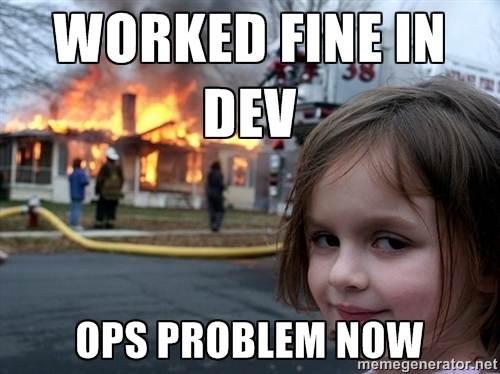
\includegraphics[width=0.45\textwidth]{images/devops.jpg}
\end{center}

This is not the case at startup companies. There isn't the money to pay for separate developers and operations teams. And in the beginning there's probably not that many servers, just a few demo systems, test systems, etc... but it spirals out from there. You're not really going to ask the sales guys to manage these servers, are you? So, there's DevOps. 

Is DevOps a good idea? Like most ideas it can be used for both good and evil. There's a lot to be said for letting the developers be involved in all the parts of the software from development to deployment to management to training the customers. Developers can learn a lot by having to do these kinds of things, and be motivated to make proper management and maintenance tools and procedures. 

There's also something to be said for never letting the developers out of their cubes and keeping them far, far away from the customers. They will be scared. Both parties.

Thanks to Chris Jones and Niall Murphy for the following points.

\subsection*{Configuration as code}
Systems have long come with complicated configuration options.
Sendmail is particularly notorious, but apache and nginx aren't super
easy to configure either.\footnote{If anyone should be foolish enough to want to look into procmail, well, good luck to you...} The first principle is to treat \emph{configuration as code}.
Therefore:
\begin{itemize}
\item use version control on your configuration.
\item test your configurations: that means that you check that they
  generate expected files, or that they spawn expected
  services. (Behaviours, or outcomes.) Also, configurations should
  ``converge''. Unlike code, they might not terminate; we're talking
  indefinitely-running services, after all. But the CPU usage should
  go down after a while, for instance.
\item aim for a suite of modular services that integrate together smoothly.
\item refactor configuration files (Puppet manifests, Chef recipes, etc);
\item use continuous builds (more on that later).
\end{itemize}

Furthermore, it's an excellent idea to have tools for configuration. It's not enough to just have a wiki page or github document titled ``How to Install AwesomeApp'' (fill in name of program here). There are tons of great tools like the Red Hat Package Manager (RPM) which will allow you to make the installation and update process automatic and simple. Complicated means mistakes... people forget steps. They are human. 

\subsection*{Servers as cattle, not pets}
By servers, I mean servers, or virtual machines, or containers.
At a certain scale (and it's smaller than you think), it's useful to
mass-produce tools for dealing with servers, rather than doing tasks
manually. At a minimum, you need to be able to set up these servers
without manual intervention. They should be able to be spun up 
programmatically.
% http://smithmeadows.com/wp-content/uploads/2012/10/Cattle.jpg

\subsection*{Common infrastructure}
Use APIs to access your infrastructure. Some examples:
\begin{itemize}
\item storage: some sort of access layer to MongoDB or Amazon S3 or whatever;
\item naming and discovery infrastructure (more below);
\item monitoring infrastructure.
\end{itemize}
Try to avoid one-offs by using, for instance, open-source tools when applicable.
Be prepared to build your own tools if needed.

\subsection*{Design for 10$\times$ growth, redesign before 100$\times$}
[original credit: Jeff Dean at Google] This discussion is based on
Martin Fowler's piece on sacrificial architecture:
\url{http://martinfowler.com/bliki/SacrificialArchitecture.html}.

Consider eBay: in 1995, perl scripts; in 1997, C++/Windows; in 2002,
Java.  Each of these architectures was appropriate at the time, but
not as the requirements change. The more sophisticated successor
architectures, however, would have been overkill at an earlier
time. And it's hard to predict what would be needed in the future.
% look up eBay growth stats
%http://martinfowler.com/bliki/images/sacrificialArchitecture/sketch.png
%http://web.archive.org/web/20000510004517/http://www.ebay.com/
% http://www.ebay.com/

\begin{quote}
``Perf is a feature''.\\
\hfill --- Jeff Atwood
\end{quote}
That is, you apply developer time to perf, and you make engineering tradeoffs
to get it. Some thoughts:
\begin{itemize}
\item design with the eventual replacement in mind;
\item don't abandon internal quality (e.g. modularity);
\item sacrifice individual modules at a time, not the whole system;
\item you can also implement new features with a rough draft and deploy to a test audience.
\end{itemize}

\subsection*{Naming}
Naming is one of the hard problems in computing. There is a saying that there are only two hard things in computers: cache invalidation, naming things, and off by one errors. 

There are a
lot of ways to name things. We'll talk about
systems/VMs\footnote{\url{http://mnx.io/blog/a-proper-naming-scheme}},
but naming is necessary for resources of all kinds.

In brief:
\begin{itemize}
\item use canonical one-word names for servers;
\item but, use aliases to specify functions, e.g. 1) geography (nyc); 2) environment (dev/tst/stg/prod); 
3) purpose (app/sql/etc); and 4) serial number.
\end{itemize}
This enables you to have a way of referring to each machine in an absolute sense, but also 
allows you to use functional names when creating dependencies between systems.

There's also the Java package approach of infinite dots: live.application.customer.webdomain.com or however you want to call it. But pick something and be consistent.

\subsection*{Other Topics}
Beyond the five principles above, there are a couple more techniques that particularly apply to
DevOps:

\paragraph{Continuous Integration.} 
This is now a best practice. It's enabled by the use of version control, good tests, and scripted deployments.
It works like this:
\begin{itemize}
\item pull code from version control;
\item build;
\item run tests;
\item report results.
\end{itemize}
What's also key is a social convention to not break the build. These things get done automatically on every commit and the results are sent to people by e-mail or instant messenger (because e-mail is for old people, right?).\footnote{I did work at a company where the person who broke the build got a sign outside his cubicle that said IOTD - Idiot of the Day. I'm not too proud to admit that I won this award on my last day of the co-op term.}

%https://jenkins-ci.org/sites/default/files/jenkins_logo.png

CI is good for all code, but it's especially good for configuration-as-code, which is especially likely
to break in different environments.

\paragraph{Canarying.}
%http://www.post-gazette.com/image/2013/10/29/ca27,76,1566,1822/Canary.jpg
Deploy new software incrementally alongside production software, also known as ``test in prod''. Sometimes
you just don't know how code is really going to work until you try it. After, of course, you use your best
efforts to make sure the code is good. Steps:
\begin{itemize}
\item stage for deployment;
\item remove canary servers from service;
\item upgrade canary servers;
\item run automatic tests on upgraded canaries;
\item reintroduce canary servers into service;
\item see how it goes!
\end{itemize}
Of course, you should implement your system so that rollback is possible.

\paragraph{Monitoring.}

Monitoring is surprisingly difficult. There are a lot of recommendations about what to monitor and what to do about it. We care about performance so here are a few things to think about:

\begin{itemize}
	\item CPU Load
	\item Memory Utilization
	\item Disk Space
	\item Disk I/O
	\item Network Traffic
	\item Clock Skew
	\item Application Response Times
\end{itemize}

With multiple systems, you will want some sort of dashboard that gives an overview of all the multiple systems in a summary. The summary needs to be sufficiently detailed that you can detect if anything is wrong, but not an overwhelming wall of data. Then you do not necessarily want to pay someone to stare at the dashboard and press the  ``Red Alert!'' button if anything goes out of some preset range of what is okay. No, for that we need some automatic monitoring.

Here's one way to think about it. 
% track down the source here: Niall Murphy interview.
\begin{itemize}
\item {\bf Alerts}: a human must take action now;
\item {\bf Tickets}: a human must take action soon (hours or days);
\item {\bf Logging}: no need to look at this except for forensic/diagnostic purposes.
\end{itemize}
A common bad situation is logs-as-tickets: you should never be in the
situation where you routinely have to look through logs to find
errors. Write code to scan logs.

It is very important to be judicious about the use of alerts. If your alerts are too common, they get ignored. When you hear the fire alarm in a building, chances are your thought is not ``the building is on fire; I should leave it immediately in an orderly fashion.''. More likely your reaction is ``great, some jerk\footnote{This is the PG-13 version of what I actually think.} has pulled the fire alarm for a stupid prank or to get out of failing a midterm.'' This is because we have been trained by far too many false alarms to think that any alarm is a false one. It's a good heuristic; you'll be correct most of the time. But if there is an actual fire, you will not only be wrong, you might also be dead.

Still, alerts and tickets are a great way to make user pain into developer pain. Being woken up in the middle of the night (... day? A lot of programmers are nocturnal, now that I think of it) because of some SUPER CRITICAL ticket OMG KITTENS ARE ENDANGERED is an excellent way to learn the lesson that production code needs to be written carefully, reviewed, QA'd, and perhaps run by a customer or two before it gets deployed to everyone. Developers, being human (... grant me some leeway here), will probably take steps to avoid their pain\footnote{There is a great quotation to this effect by Fr\'ed\'eric Bastiat about how men will avoid pain and work is pain.}. and they will take steps that keep these things from happening in the future: good processes and monitoring and all that goes with it.

\section*{Clusters versus Laptops}
There is a paper about this: Frank McSherry, Michael Isard, Derek G. Murray. ``Scalability! But at what COST?'' HotOS XV. This part of the lecture is based on the companion blog post~\cite{scalecost}.

The key idea: scaling to big data systems introduces substantial overhead. Let's just see how, say, a laptop compares, in absolute times, to 128-core big data systems.

\paragraph{Summary.} Big data systems haven't yet been shown to be obviously good; current evaluation is lacking.
The important metric is not just scalability; absolute
performance matters a lot too. We don't want a situation where we are just scaling up to $n$ systems to deal with the complexity of scaling up to $n$ systems. Or, as Oscar Wilde put it: ``The bureaucracy is expanding to meet the needs of the expanding bureaucracy.''

\paragraph{Methodology.} We'll compare a competent single-threaded implementation to top
big data systems, as described in an OSDI 2014 (top OS conference) paper on GraphX\cite{graphx}. The domain: graph processing
algorithms, namely PageRank and graph connectivity (for which the bottleneck is label propagation). The subjects: graphs with billions of edges, amounting to a few
GB of data.

\paragraph{Results.} 128 cores don't consistently beat a laptop at PageRank: e.g. 249--857s on the twitter\_rv dataset for the big data system vs 300s for the laptop, and they are 2$\times$ slower for label
propagation, at 251--1784s for the big data system vs 153s on
twitter\_rv. From the blogpost:

\begin{center}
	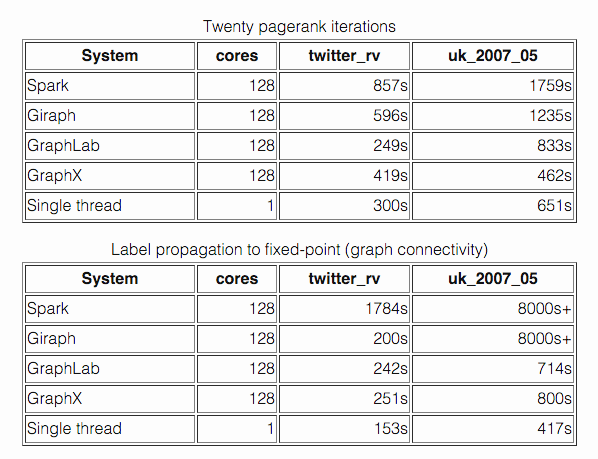
\includegraphics[width=0.60\textwidth]{images/pagerank.png}
\end{center}

\paragraph{Wait, there's more.} I keep on saying that we can improve algorithms for additional performance boosts too.
But that doesn't generalize, so it's hard to teach. In this case, two improvements are: using Hilbert curves
for data layout, improving memory locality, which helps a lot for PageRank; and using a union-find algorithm 
(which is also parallelizable). ``10$\times$ faster, 100$\times$ less embarrassing''.  We observe an overall
$2\times$ speedup for PageRank and $10\times$ speedup for label propagation.

\paragraph{Takeaways.} Some thoughts to keep in mind, from the authors:
\begin{itemize}
\item    ``If you are going to use a big data system for yourself, see if it is faster than your laptop.''
\item    ``If you are going to build a big data system for others, see that it is faster than my laptop.''
\end{itemize}



\bibliographystyle{alphaurl}
\bibliography{459}


\end{document}
